\section{Résultats}

\begin{minipage}{\textwidth}
    \begin{wrapfigure}{R}{0.6\textwidth}
        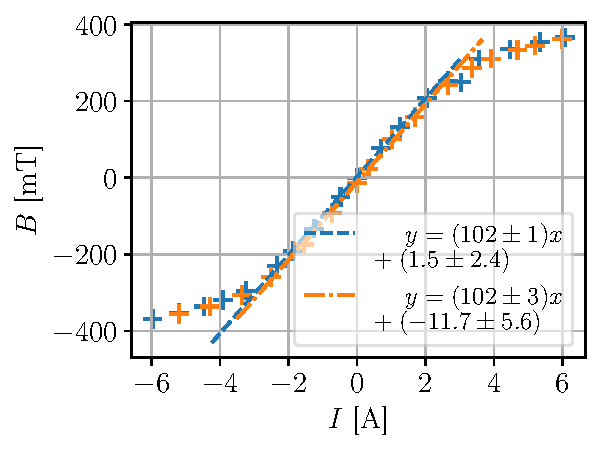
\includegraphics[width=\linewidth]{figures/calibration.pdf}
        \caption{Variation de l'amplitude du champ magnétique en fonction du courant sur un cycle \(I_\textrm{max} -> \)}
    \end{wrapfigure}

    \paragraph*{Étalonnage du champ d'induction}
    Regarde c'est pas hyper linéaire

    Eu voluptate nisi esse cupidatat excepteur consequat ea laboris ad eu. Incididunt duis excepteur Lorem elit aliquip Lorem dolore velit labore esse. Eiusmod deserunt elit non nisi excepteur id quis aliqua ut amet ea dolor labore velit. Non dolore velit ex qui aliqua elit consequat. Dolore elit fugiat irure incididunt ex est. Magna anim mollit esse officia occaecat Lorem minim incididunt veniam et velit adipisicing incididunt in.

    Ad aliqua pariatur aliquip mollit est in nulla veniam. Qui dolor commodo aute laborum irure officia est. Adipisicing quis occaecat esse adipisicing exercitation nulla sint culpa ad veniam. Excepteur est Lorem Lorem irure nostrud eiusmod. Minim culpa non anim commodo aute in dolor. Duis Lorem dolore incididunt ullamco amet sit.

    Occaecat ipsum adipisicing aute sit Lorem. Ea nisi mollit velit cillum incididunt duis. Labore pariatur tempor et tempor anim sit aute commodo mollit deserunt sunt est non mollit. Occaecat aliqua nostrud do sit duis nostrud.
\end{minipage}

\paragraph*{Mesure des tensions résiduelles pour InP}
Blabla regarde tension résiduelle pour un courant nul \autoref{tab:tension_residuelle}

\begin{table}[h]
    \centering
    \begin{tabulary}{\textwidth}{C C C C}
        \toprule
        Configuration \si{\micro\meter} & Tension (\(a = 1\) \si{\micro\meter}) [\si{\milli\volt}] & Tension (\(a = 2\) \si{\micro\meter}) [\si{\milli\volt}] \\
        \midrule
        \(I_{13}U_{24}\) & \(68.74 \pm 0.01\) & \(27.02 \pm 0.01\) \\
        \(I_{31}U_{42}\) & \(68.69 \pm 0.01\) & \(27.12 \pm 0.01\) \\
        \(I_{24}U_{13}\) & \(39.93 \pm 0.01\) & \(24.78 \pm 0.01\) \\
        \(I_{42}U_{31}\) & \(40.12 \pm 0.01\) & \(24.76 \pm 0.01\) \\
        \bottomrule
    \end{tabulary}
    \caption{Tension résiduelle pour différentes configuration et 2 épaisseurs de l'échantillon InP}
    \label{tab:tension_residuelle}
\end{table}

\paragraph*{Détermination de la constante de Hall pour InP}
Regarde ces belles relations linéaires uwu

On trouve pour 1µm \(R_H = (2.40 \pm 0.05) \cdot 10^{-3}\) \si{\meter\cubed\per\coulomb} et \(N = (2.60 \pm 0.05) \cdot 10^{21}\) \si{\per\meter\cubed}

On trouve pour 2µm \(R_H = (1.47 \pm 0.03) \cdot 10^{-3}\) \si{\meter\cubed\per\coulomb} et \(N = (4.25 \pm 0.08) \cdot 10^{21}\) \si{\per\meter\cubed}

\begin{figure}[h]
    \centering
    \begin{subfigure}{0.45\textwidth}
        \centering
        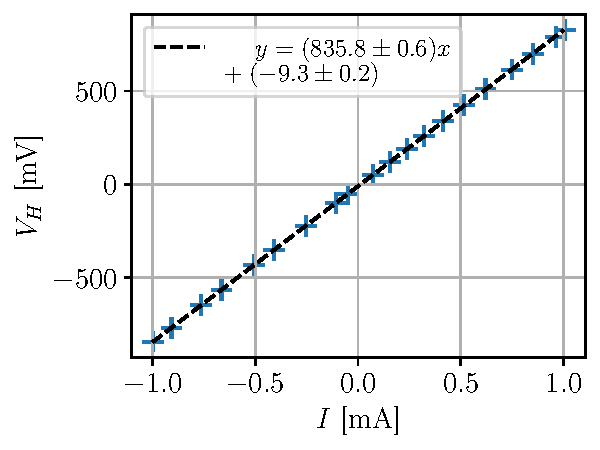
\includegraphics[width=\textwidth]{figures/U(I),InP1micro.pdf}
        \caption{}
    \end{subfigure}
    \begin{subfigure}{0.45\textwidth}
        \centering
        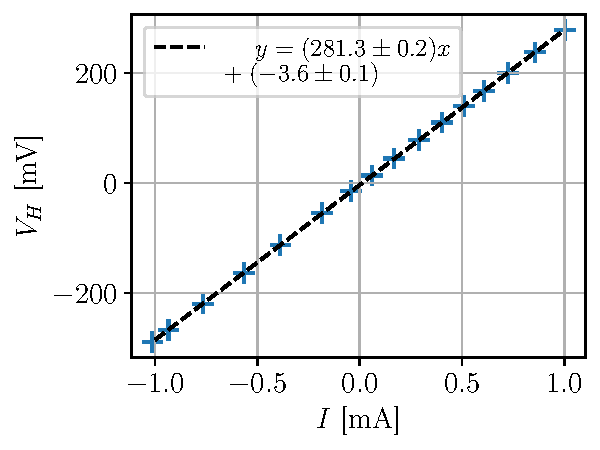
\includegraphics[width=\textwidth]{figures/U(I),InP2micro.pdf}
        \caption{}
    \end{subfigure}
    \caption{Tension en fonction de l'intensité pour l'échantillon InP d'épaisseur (a) 1 \si{\micro\meter} (b) 2 \si{\micro\meter}}
\end{figure}

\begin{figure}[h]
    \centering
    \begin{subfigure}{0.45\textwidth}
        \centering
        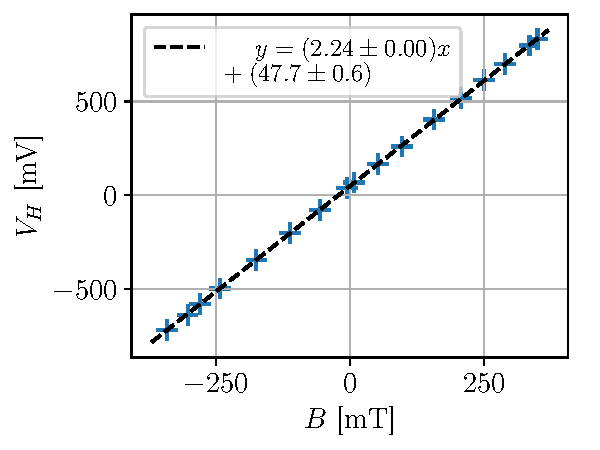
\includegraphics[width=\textwidth]{figures/U(B),InP1micro.pdf}
        \caption{}
    \end{subfigure}
    \begin{subfigure}{0.45\textwidth}
        \centering
        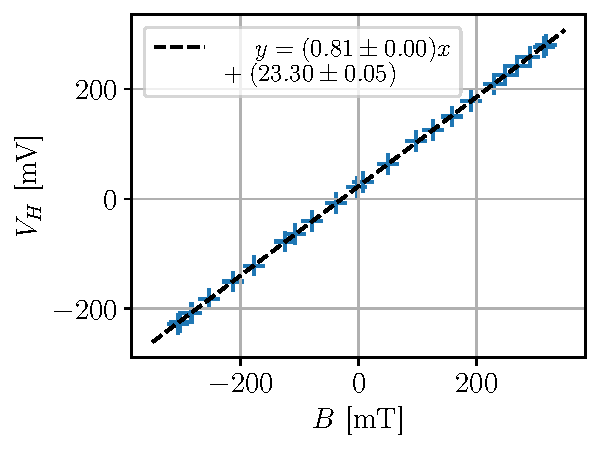
\includegraphics[width=\textwidth]{figures/U(B),InP2micro.pdf}
        \caption{}
    \end{subfigure}
    \caption{Tension en fonction de la norme signée du champ magnétique pour l'échantillon InP d'épaisseur (a) 1 \si{\micro\meter} (b) 2 \si{\micro\meter}}
\end{figure}
